% Author: Izaak Neutelings (May 2021)
% Description: hadronic top quark jet
\documentclass[border=3pt,tikz]{standalone}
\usepackage{amsmath}
\usepackage{physics}
\usepackage{xcolor}
\usetikzlibrary{calc}
\usetikzlibrary{math} % for \tikzmath
\tikzset{>=latex} % for LaTeX arrow head
\usetikzlibrary{decorations.pathreplacing} % for curly braces

\colorlet{myblue}{blue!70!black}
\colorlet{mydarkblue}{blue!40!black}
\colorlet{mygreen}{green!40!black}
\colorlet{myred}{red!65!black}
\tikzstyle{cone}=[thin,blue!50!black,fill=blue!50!black!30] %,fill opacity=0.8
\tikzstyle{conebase}=[cone,fill=blue!50!black!50] %,fill opacity=0.8

\newcommand\jetcone[5][blue]{{
  \pgfmathanglebetweenpoints{\pgfpointanchor{#2}{center}}{\pgfpointanchor{#3}{center}}
  \edef\ang{#4/2}
  \edef\e{#5}
  \edef\vang{\pgfmathresult} % angle of vector OV
  \tikzmath{
    coordinate \C;
    \C = (#2)-(#3);
    \x = veclen(\Cx,\Cy)*\e*sin(\ang)^2; % x coordinate P
    \y = tan(\ang)*(veclen(\Cx,\Cy)-\x); % y coordinate P
    \a = veclen(\Cx,\Cy)*sqrt(\e)*sin(\ang); % vertical radius
    \b = veclen(\Cx,\Cy)*tan(\ang)*sqrt(1-\e*sin(\ang)^2); % horizontal radius
    \angb = acos(sqrt(\e)*sin(\ang)); % angle of P in ellipse
  }
  \coordinate (tmpL) at ($(#3)-(\vang:\x pt)+(\vang+90:\y pt)$); % tangency
  \draw[thin,#1!40!black,rotate=\vang, %,fill=#1!50!black!80
    top color=#1!50!black!80,bottom color=#1!40!black!80,shading angle=\vang]
    (#3) ellipse({\a pt} and {\b pt});
  \draw[thin,#1!40!black,rotate=\vang,%fill=#1!80!black!40,
  top color=#1!90!black!20,bottom color=#1!50!black!50,shading angle=\vang]
    (tmpL) arc(180-\angb:180+\angb:{\a pt} and {\b pt})
    -- ($(#2)+(0.018,0)$) -- cycle;
}}


\begin{document}


% RESOLVED TOP JETS
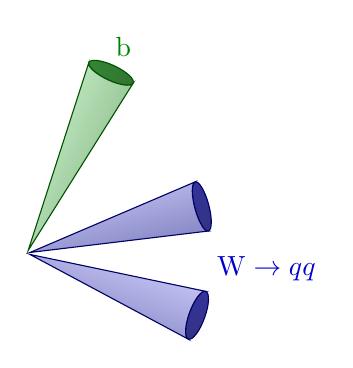
\begin{tikzpicture}[scale=2.3]
  \coordinate (O) at (0,0);
  \coordinate (BJ) at ( 65:1.1); % b jet 1
  \coordinate (J1) at ( 15:1.0); % q jet 1
  \coordinate (J2) at (-20:1.0); % q jet 2
  \jetcone[green!80!black]{O}{BJ}{14}{0.10}
  \jetcone{O}{J1}{16}{0.08}
  \jetcone{O}{J2}{16}{0.10}
  \node[green!50!black] at (65:1.26) {b};
  \node[blue!80!black,right] at (-5:1.00) {$\mathrm{W} \to qq$};
\end{tikzpicture}


% BOOSTED TOP JETS, partially merged
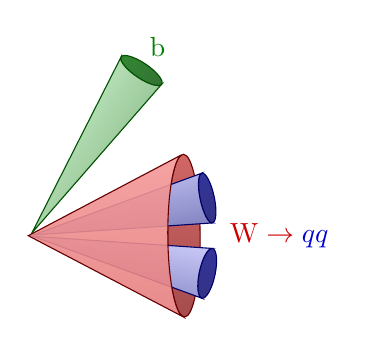
\begin{tikzpicture}[scale=2.3]
  \edef\ang{28}
  \edef\e{0.05}
  \coordinate (O) at (0,0);
  \coordinate (BJ) at ( 56:1.1); % b jet 1
  \coordinate (J1) at ( 12:1.0); % q jet 1
  \coordinate (J2) at (-12:1.0); % q jet 2
  \coordinate (M) at (0:0.85); % merged
  \edef\vang{\pgfmathresult} % angle of vector OV
  \tikzmath{
    coordinate \C;
    \C = (O)-(M);
    \x = veclen(\Cx,\Cy)*\e*sin(\ang)^2; % x coordinate P
    \y = tan(\ang)*(veclen(\Cx,\Cy)-\x); % y coordinate P
    \a = veclen(\Cx,\Cy)*sqrt(\e)*sin(\ang); % vertical radius
    \b = veclen(\Cx,\Cy)*tan(\ang)*sqrt(1-\e*sin(\ang)^2); % horizontal radius
    \angb = acos(sqrt(\e)*sin(\ang)); % angle of P in ellipse
  }
  \coordinate (ML) at ($(M)+(\vang-180:\x pt)+(\vang+90:\y pt)$); % tangency
  
  % JETS
  \draw[thin,red!40!black,rotate=\vang, %,fill=red!70!black!60
        top color=red!70!black!60,bottom color=red!50!black!70,shading angle=\vang] % base
    (M) ellipse({\a pt} and {\b pt});
  \jetcone[green!80!black]{O}{BJ}{14}{0.10}
  \jetcone{O}{J1}{16}{0.08}
  \jetcone{O}{J2}{16}{0.10}
  \draw[thin,red!40!black,fill opacity=0.9,rotate=\vang, %,fill=red!90!black!40
        top color=red!90!black!40,bottom color=red!80!black!50,shading angle=\vang]
    (ML) arc(180-\angb:180+\angb:{\a pt} and {\b pt})
    -- ($(O)-(0.01,0)$) -- cycle;
  
  \node[green!50!black] at (56:1.26) {b};
  \node[blue!80!black,right] at (0:1.05) {${\color{red!80!black}\mathrm{W} \to}\; qq$};
\end{tikzpicture}


% BOOSTED TOP JETS, fully merged
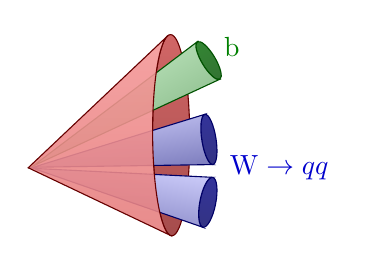
\begin{tikzpicture}[scale=2.3]
  \edef\ang{35}
  \edef\e{0.05}
  \coordinate (O) at (0,0);
  \coordinate (BJ) at ( 31:1.15); % b jet 1
  \coordinate (J1) at (  9:1.00); % q jet 1
  \coordinate (J2) at (-11:1.00); % q jet 2
  \coordinate (M) at (13:0.80); % merged
  \edef\vang{\pgfmathresult} % angle of vector OV
  \tikzmath{
    coordinate \C;
    \C = (O)-(M);
    \x = veclen(\Cx,\Cy)*\e*sin(\ang)^2; % x coordinate P
    \y = tan(\ang)*(veclen(\Cx,\Cy)-\x); % y coordinate P
    \a = veclen(\Cx,\Cy)*sqrt(\e)*sin(\ang); % vertical radius
    \b = veclen(\Cx,\Cy)*tan(\ang)*sqrt(1-\e*sin(\ang)^2); % horizontal radius
    \angb = acos(sqrt(\e)*sin(\ang)); % angle of P in ellipse
  }
  \coordinate (ML) at ($(M)+(\vang-180:\x pt)+(\vang+90:\y pt)$); % tangency
  
  % JETS
  \draw[thin,red!40!black,rotate=\vang, %,fill=red!70!black!60
        top color=red!70!black!60,bottom color=red!50!black!70,shading angle=\vang] % base
    (M) ellipse({\a pt} and {\b pt});
  \jetcone[green!80!black]{O}{BJ}{12}{0.10}
  \jetcone{O}{J1}{16}{0.08}
  \jetcone{O}{J2}{16}{0.10}
  \draw[thin,red!40!black,fill opacity=0.9,rotate=\vang, %,fill=red!90!black!40
        top color=red!90!black!40,bottom color=red!80!black!50,shading angle=\vang]
    (ML) arc(180-\angb:180+\angb:{\a pt} and {\b pt})
    -- ($(O)-(0.01,0)$) -- cycle;
  
  \node[green!50!black] at (31:1.3) {b};
  \node[blue!80!black,right] at (0:1.05) {$\mathrm{W} \to qq$};
\end{tikzpicture}


\end{document}